\documentclass[10pt]{article}
\usepackage{kotex}
\usepackage[margin=0.6in]{geometry} % set the margins to 1in on all sides
\usepackage{graphicx} % to include figures
\usepackage{amsmath} % great math stuff
\usepackage{amsfonts} % for blackboard bold, etc
\usepackage{amsthm} % better theorem environments
\usepackage{amssymb}
\usepackage[utf8]{inputenc}
\usepackage{booktabs}
\usepackage{array}
\usepackage{courier}
\usepackage[usenames, dvipsnames]{color}
\usepackage{titlesec}
\usepackage{empheq}
\usepackage{tikz}
\usepackage{wrapfig}
\usepackage{float}

\linespread{1.5}

\newcommand\encircle[1]{%
  \tikz[baseline=(X.base)] 
    \node (X) [draw, shape=circle, inner sep=0] {\strut #1};}
 
% Command "alignedbox{}{}" for a box within an align environment
% Source: http://www.latex-community.org/forum/viewtopic.php?f=46&t=8144
\newlength\dlf  % Define a new measure, dlf
\newcommand\alignedbox[2]{
% Argument #1 = before & if there were no box (lhs)
% Argument #2 = after & if there were no box (rhs)
&  % Alignment sign of the line
{
\settowidth\dlf{$\displaystyle #1$}  
    % The width of \dlf is the width of the lhs, with a displaystyle font
\addtolength\dlf{\fboxsep+\fboxrule}  
    % Add to it the distance to the box, and the width of the line of the box
\hspace{-\dlf}  
    % Move everything dlf units to the left, so that & #1 #2 is aligned under #1 & #2
\boxed{#1 #2}
    % Put a box around lhs and rhs
}
}


\newtheorem{thm}{Theorem}[section]
\newtheorem{lem}[thm]{Lemma}
\newtheorem{prop}[thm]{Proposition}
\newtheorem{cor}[thm]{Corollary}
\newtheorem{conj}[thm]{Conjecture}

\setcounter{secnumdepth}{4}

\titleformat{\paragraph}
{\normalfont\normalsize\bfseries}{\theparagraph}{1em}{}
\titlespacing*{\paragraph}
{0pt}{3.25ex plus 1ex minus .2ex}{1.5ex plus .2ex}

\definecolor{myblue}{RGB}{72, 165, 226}
\definecolor{myorange}{RGB}{222, 141, 8}

\setlength{\heavyrulewidth}{1.5pt}
\setlength{\abovetopsep}{4pt}


\DeclareMathOperator{\id}{id}
\DeclareMathOperator{\argmin}{\arg\!\min}
\DeclareMathOperator{\Tr}{Tr}

\newcommand{\bd}[1]{\mathbf{#1}} % for bolding symbols
\newcommand{\RR}{\mathbb{R}} % for Real numbers
\newcommand{\ZZ}{\mathbb{Z}} % for Integers
\newcommand{\col}[1]{\left[\begin{matrix} #1 \end{matrix} \right]}
\newcommand{\comb}[2]{\binom{#1^2 + #2^2}{#1+#2}}
\newcommand{\bs}{\boldsymbol}
\newcommand{\opn}{\operatorname}
\begin{document}
\nocite{*}

\title{$\pi$에 관하여}
\author{임대영 \\ 고려대학교 통계학과}
\maketitle

\section{도입부: 수학과 철학}
단언컨대 대부분의 사람들은 수학이 절대적인 진리의 영역이라 생각할 것이다. 이 믿음은 시간을 거슬러 올라가 고대 피타고라스에서도 찾아볼 수 있다. 세상 삼라만상의 진리는 숫자로부터 나오며 수를 아는 것이 곧 진리를 아는 것이라 믿는 사람들. 만물의 근원, 즉 `아르케(arche)'를 찾으려는 노력은 그 대상이 바뀌어, 인간세계의 아르케, 즉 자아와 규범을 찾기에 이른다. 근대에 이르러서는 수학의 깊이가 더욱 깊어져 많은 것을 표현하는 하나의 체계가 구축된다. 하지만 여전히 의문은 남아있다. 인간은 진정한 `앎'에 도달할 수 있는가.\par
이 물음에 답하려 했던 사람 중 르네 데카르트가 있다. 근대 철학의 본질이 된 ``나는 생각한다. 고로 존재한다.''라는 선언은 아이러니하게도 근대 철학의 딜레마를 상징하게 되었다. 생각하는 내가 존재하는 것은 자명하지만 나를 제외한 나머지, 타자를 인식하는 것은 불가능한 세상이 되었다. 진리를 탐구하는 과학의 영역에서 확실한 게 없어지다니, 참담한 현실이다. 데카르트의 방법론처럼 이제는 진리에 가까이 가기 위해 끝없이 의심하고 철저한 불신으로 일관해야 했다. 그리고 마침내 프랑스의 철학자 미셸 푸코가 제시한 대로 `반박가능성(falsifiability)'가 없는 것은 과학적 탐구의 대상이 아닌 것이 되었다. 불확실성이 없는 것은 진리가 될 수 없다는 매우 역설적인 선언이었다. \par
이러한 세계에 우리는 살고 있다. 여기서 수학은 매우 중요한 도구가 된다. 흔히 과학을 하는 사람들은 `모델링'을 한다고 한다. 수학은 현실 세계를 매우 잘 `모델링'한 체계성을 갖춘 도구이다. 그 말은 수학이 현실이 아니라는 말이다. 수학은 사람들이 부여한 규칙 속에서 쌓아올려진 한 가지 시스템일 뿐이다. 그 규칙을 바꾸면 전체적인 시스템도 바뀌게 된다 --- 척도 이론(Measure Theory)에서 수학의 이러한 특징이 여실히 드러난다---. $\pi$도 역시 수학의 테두리 안에 있는 하나의 창조물이다. 우리가 흔히 말하는 `원주율'은 가상의 개념일 뿐이다. 그 어떤 물리적으로 존재하는 원과 물리적으로 존재하는 지름의 비도 정확히 $\pi$와 일치하지 않는다. 모든 물리적 측정에는 오차가 존재하기 마련이기 때문이다. 피타고라스는 인간이 만들어낸 도구를 신으로 추대했다. 그리고 그 믿음의 잔재가 여전히 이 사회 속 사람들에게 남아있다. 위와 같은 철학적 흐름과 근대 사회에서 과학이 차지하는 위치가 어떤지, 그리고 그속에서 수학은 어떤 역할을 하는 것인지 이해하지 않으면 수학에 대한 절대적 믿음이 생기게 된다. 그 이해 속에서 $\pi$라는 숫자를 파헤쳐 보도록 하자.

\section{$\pi$의 정의}
\subsection{지금까지의 파이는 잘못됐다!}
\begin{wrapfigure}{r}{0.2\textwidth}
  \centering
  
\includegraphics[width = 0.2\textwidth]{exp_mosaic.png}
\end{wrapfigure}\par
한국에서 고등 교육을 받은 사람이라면 $\pi$를 모르는 사람은 없을 것이다. 하지만 매일 $\pi$를 써서 계산을 해 내는 물리학자나 수학자도 $\pi$에 대해 설명하라고 하면 단박에 그 정수를 찔러 설명하지 못할 듯싶다. 그토록 이 숫자에는 아주 중요한 성질이 있고 그것은 한 마디로 표현하기에는 너무 중요하다.\par
$\pi$는 원주율이다. 분명 이 숫자는 원과 관련이 있다. 그러나 이러한 정의는 `틀렸다'고 할 수 있을 정도로 그 본질을 설명하지 못한다. $\pi$는 원이나 각도 따위를 알지 못한다. 예를 들어, 통계학에서 가장 중요한 정규 분포의 밀도 함수에 등장하는 $1/\sqrt{2\pi}$에서 원의 흔적을 발견할 수 있는가? 원의 성질과 연결시키지 않아도 우리는 충분히 정규 분포의 중요성을 설명할 수 있다. 왜냐하면 $\pi$는 원에서 나온 숫자가 아니기 때문이다. $\pi$는 원과 관련짓지 않고도 그 중요성을 명료하게 설명할 수 있는 숫자이다.\par
\begin{wrapfigure}{l}{0.5\textwidth}
  \centering
  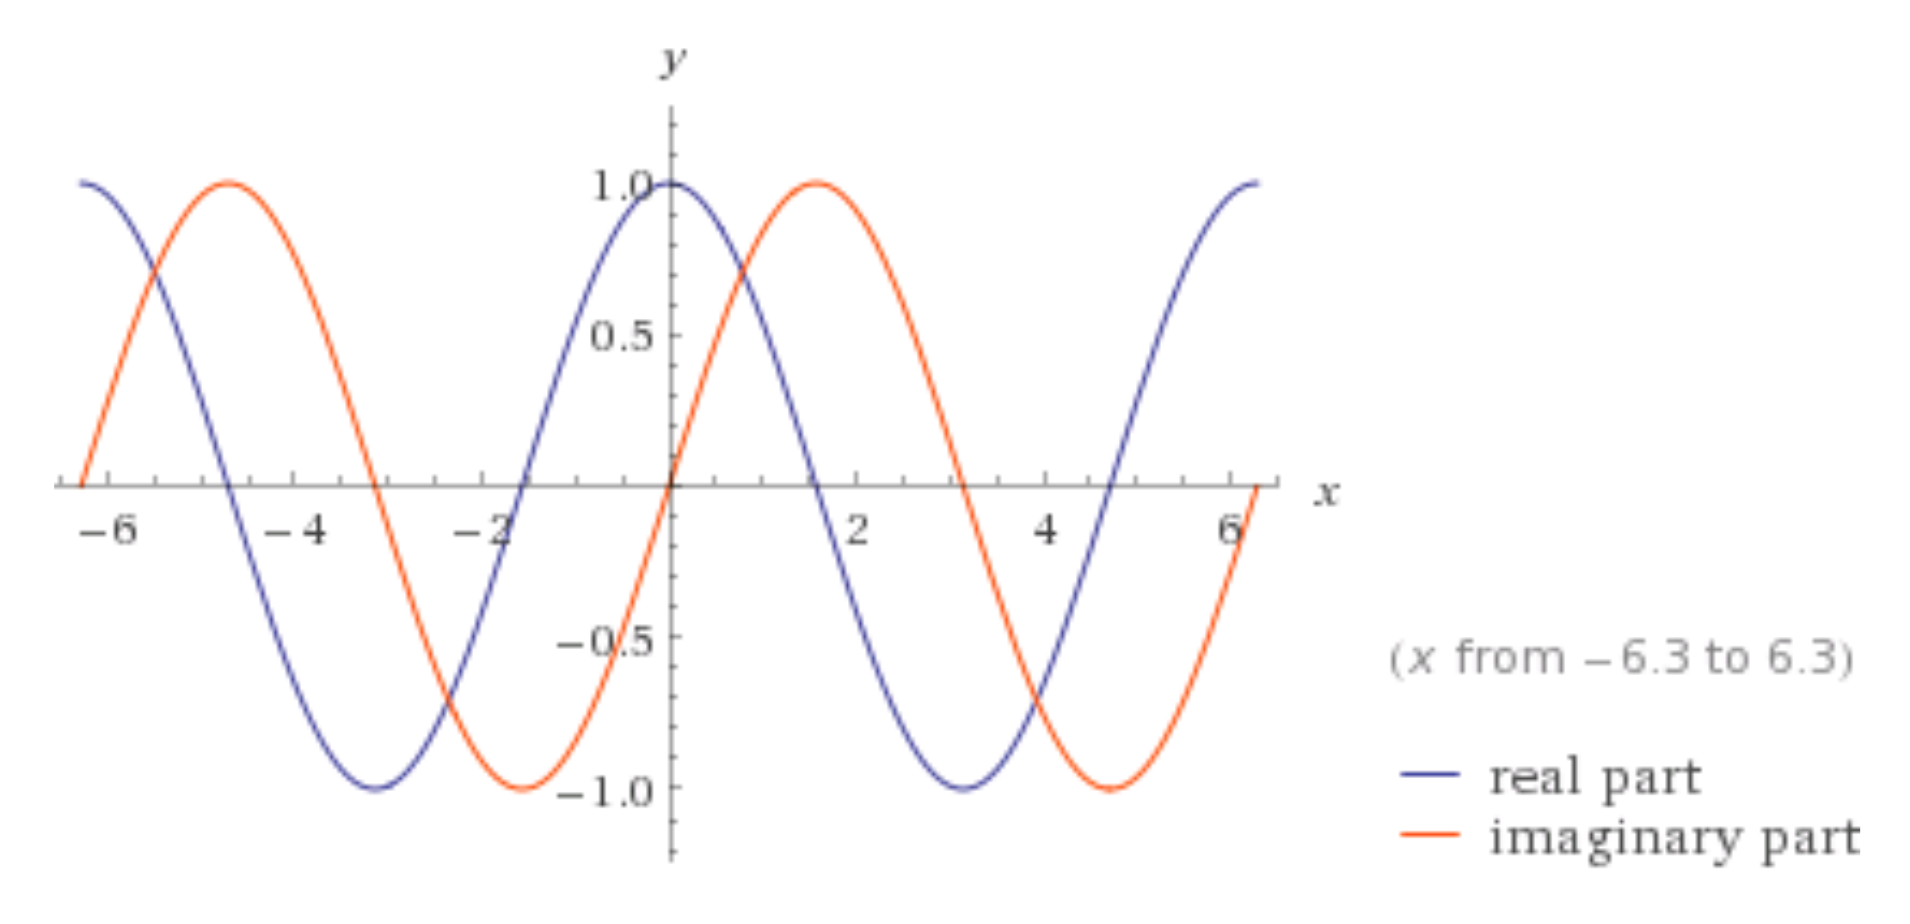
\includegraphics[width = 0.5\textwidth]{exponential.png}
\end{wrapfigure}
그렇다면 도대체 이 간단하고도 엄청나 보이는 숫자는 어떻게 해서 등장하게 된 것일까? 답은 바로 `지수 함수'에 있다. 복소 공간에서 지수 함수의 행적을 잘 살펴보면 $\pi$의 모습이 보일 것이다. 믿기지 않는가? 위의 그림을 보자. 이 그림은 $\exp\left(ix\right)$의 모자이크 이미지이다.
색깔이 반복되는 것을 보면 지수 함수가 어떠한 주기를 가지고 있음을 알 수 있다. 더 자세하게 보려면 복소 공간에서의 지수 함수를 실수부와 허수부를 따로 표현한 왼쪽의 그래프를 보아라. 예상했듯이 주기성을 보이고 있다. 지수 함수는 수학 문제를 풂에 있어서 도처에 나타나는데, 그 보편성은 다음의 미분방정식이 가장 기본이 모든 문제에서 가장 단순하고도 근간이 되기 때문이다.
$$
  f' = f
$$
단순하기 그지없는 이 방정식이 만물의 움직임을 나타내는 미분 방적식의 기저에 깔려 있다니! 매우 놀라운 일이다. 이 방정식을 분석하다보면 자연스럽게 $\pi$와 $e$를 정의할 수 있게 된다. 

\end{document}


